\documentclass[border=2mm]{standalone}
\usepackage{tikz,pgfplots}
\pgfplotsset{compat=1.11}
\begin{document}
\begin{tabular}{cc}

  \begin{tikzpicture}
    \begin{axis}[
  xtick={0,1/6,...,1},
  ytick={0,1/6,...,1}, grid,
  xmin=0,   xmax=1,
  ymin=0,   ymax=1,scale=1,
  xlabel= \textbf{$r_1=1/6\quad $} \textbf{$N(r_1)=23$},
  xticklabels=\empty,
  yticklabels=\empty] 
      \addplot[thick,blue] graphics[xmin=0,ymin=0,xmax=1,ymax=1] {spain3.png};
    \end{axis}
  \end{tikzpicture}
&  
  \begin{tikzpicture}
    \begin{axis}[
  xtick={0,1/12,...,1},
  ytick={0,1/12,...,1}, grid,
  xmin=0,   xmax=1,
  ymin=0,   ymax=1,scale=1,
  xlabel= \textbf{$r_2=1/12\quad $} \textbf{$N(r_2)=52$},
  xticklabels=\empty,
  yticklabels=\empty] 
      \addplot[thick,blue] graphics[xmin=0,ymin=0,xmax=1,ymax=1] {spain3.png};
    \end{axis}
  \end{tikzpicture}  
\\  
    \begin{tikzpicture}
    \begin{axis}[
  xtick={0,1/24,...,1},
  ytick={0,1/24,...,1}, grid,
  xmin=0,   xmax=1,
  ymin=0,   ymax=1,scale=1,
  xlabel= \textbf{$r_3=1/24\quad $} \textbf{$N(r_3)=121$},
  xticklabels=\empty,
  yticklabels=\empty] 
       \addplot[thick,blue] graphics[xmin=0,ymin=0,xmax=1,ymax=1] {spain3.png};
    \end{axis}
  \end{tikzpicture} 
  &
 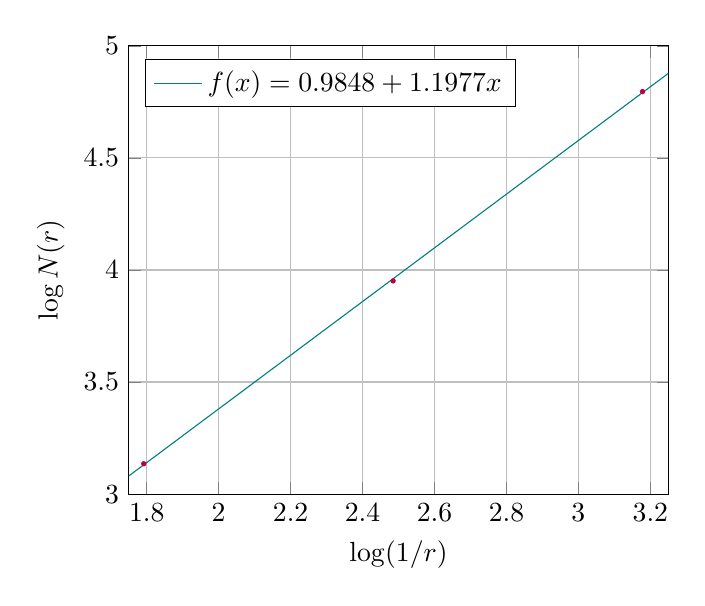
\begin{tikzpicture}
    \begin{axis}[legend pos=north west,
    samples=50, 
    domain=1.75:3.25, 
    ymin=3,
    ymax=5,
    xmin=1.75, 
    xmax=3.25, 
    xlabel=$\log(1/r)$,
    ylabel=$\log N(r)$, 
    grid=major,scale=1]
      \addplot [blue!50!green,smooth, thin] {0.984793 + 1.197651*x};  
      \addplot[purple,only marks,mark size=0.75pt] coordinates {
       (1.7918, 3.1355)
       (2.4849, 3.9512)
       (3.1781, 4.7958)
        }; 
       \legend{$f(x)=0.9848 + 1.1977x$}   
     \end{axis}
\end{tikzpicture} 
\end{tabular}
\end{document}
